\section{Introduction}
Temporal Networks scheduling algorithms support diverse formulations useful in modeling practical problems. Examples include dynamical execution strategies based on partial knowledge of uncertain durations, and strategies to upper-bound the probability of failing to satisfy temporal constraints given distributions over uncertain durations. However, it is not obvious how to apply them in scenarios with resource usage constraints. While some prior work exists in operations research literature, known as project scheduling or job-shop scheduling, much of the focus is on discrete resources. We attempt to narrow the gap between the two independent bodies of work.

As a motivating example, consider the following Smart House scenario. A $150W$ generator is available, and we know that the resident returns home at some time defined by a Normal distribution $N(5pm, 5minutes)$. Moreover we know that sun sets at time defined by $N(7pm, 1minute)$. We would like to meet the following constraints with the overall probability at least $98\%$:
\begin{itemize}
\setlength\itemsep{0.00em}

\item Wash clothes (duration: $2hours$, power usage: $130W$) before user comes back from work
\item Cook dinner (duration: $30minutes$, power usage: $100W$) ready within 15 minutes of user coming back from work
\item Have the lights on (power usage: $80W$) from before sunset to at least midnight.
\item Cook a late night snack (duration: $30minutes$, power usage: $20W$) between 10pm and 11pm.
\end{itemize}
While probabilistic constraints can be  modeled using probabilistic Simple Temporal Networks \cite{Fang2014} and solved accordingly, there is no known model which captures the tightly coupled resource constraints. 

In this paper, we introduce the Time Resource Network (TRN), a general framework capable of encoding scenarios similar to the example described. We describe two algorithms which schedules resource usage given TRN models, one based on a standard encoding as a mixed integer linear program (MILP) and a novel algorithm leveraging prior specialized algorithms for solving temporal problems. Using the algorithms, we are able to derive a solution to the above example which meets the constraints with $99.7\%$ probability (presented on Figure \ref{fig:pstnu_scheduling}). We also show through benchmarking that the novel algorithm is significantly faster even when the MILP encoding is solved with state-of-the-art commercial solvers. 


\begin{figure}[H]
\begin{center}
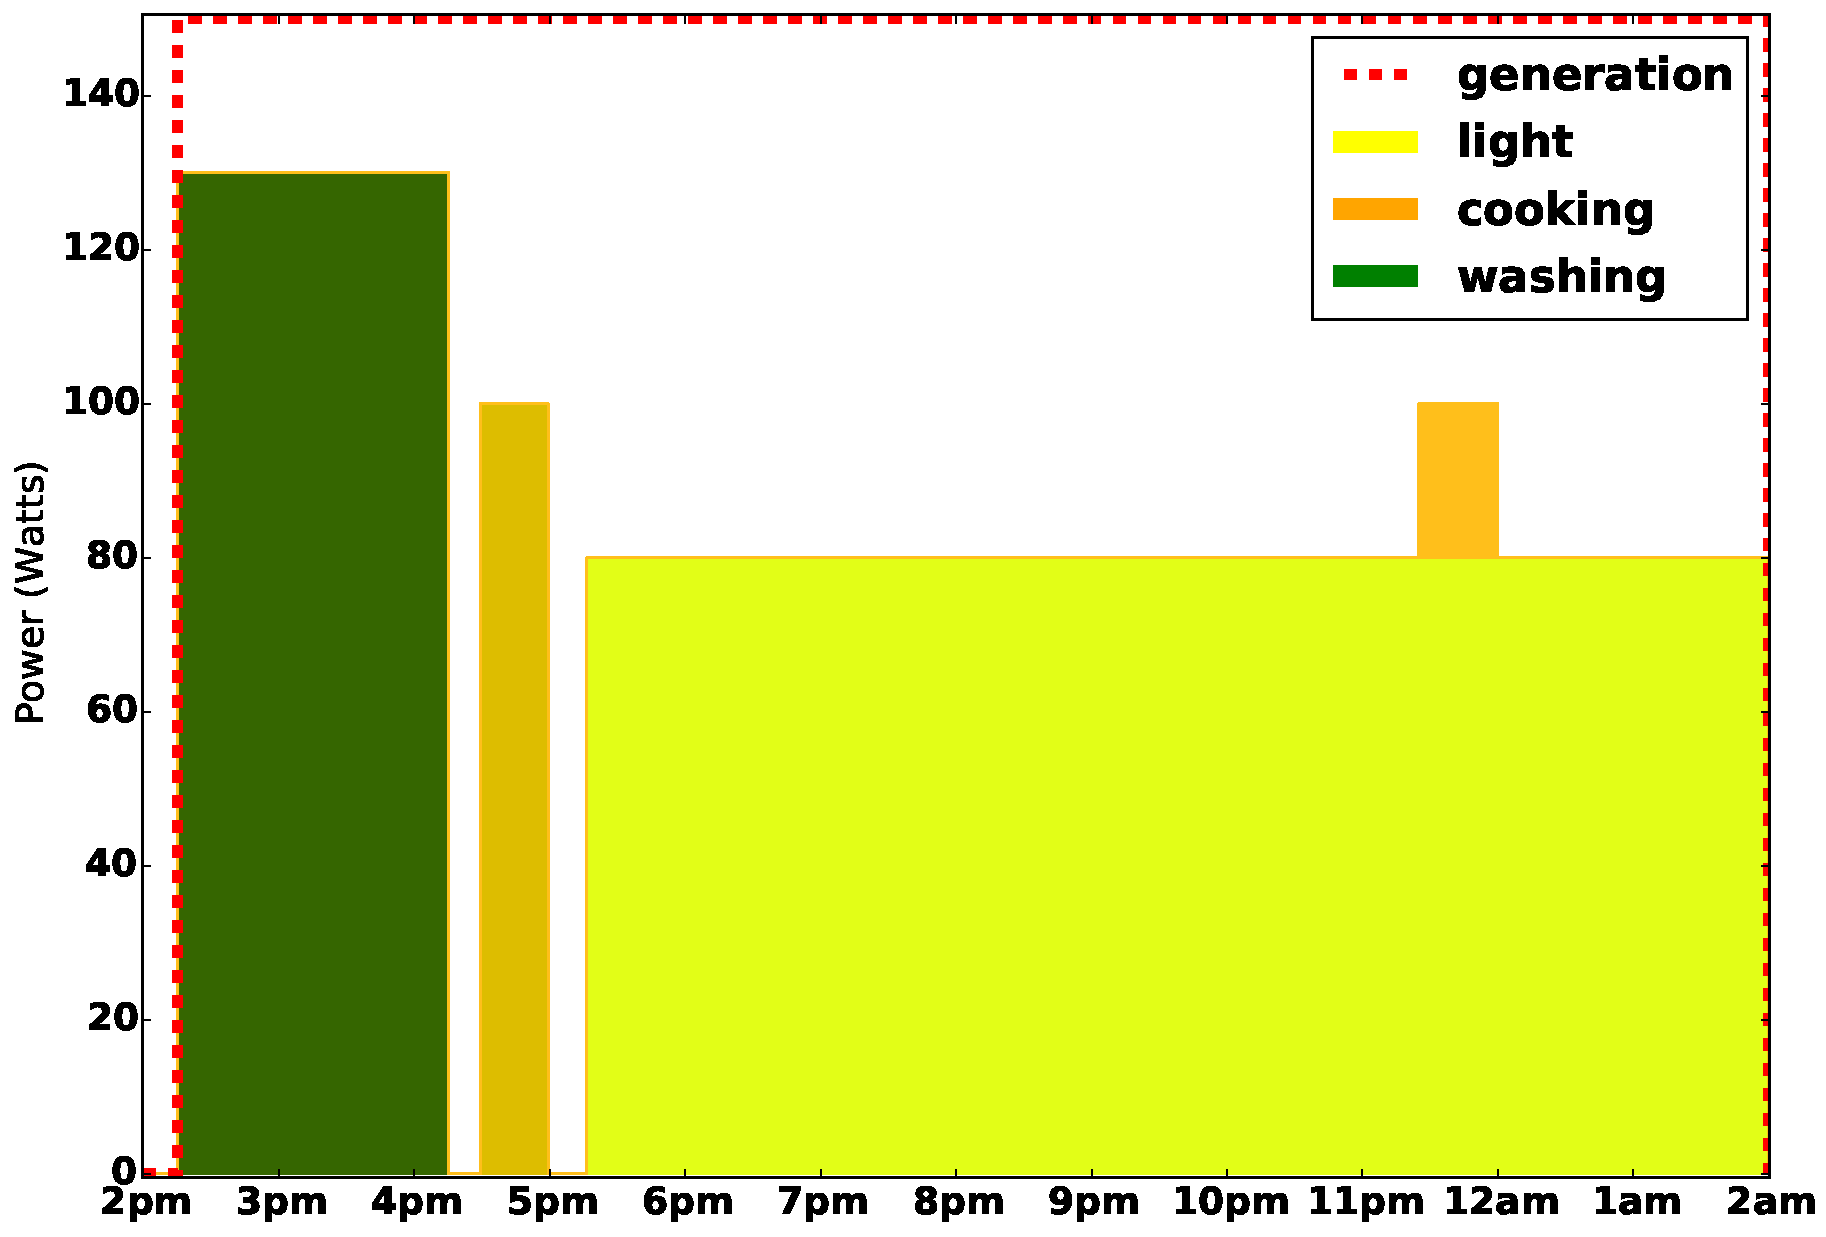
\includegraphics[width=0.4\textwidth]{pstnu_scheduling}
\caption{Depiction of solution to TRN spanning a pSTN.}
\label{fig:pstnu_scheduling}
\end{center}
\end{figure}
